\subsection{Terugvoer onderdeel}

Die terugvoer onderdeel maak dit moontlik vir gebruikers om terugvoer oor
maaltye en dienste te verskaf, en vir administrateurs om hierdie terugvoer te
bestuur en te analiseer. Dit sluit die insameling van graderings en
kommentaar, asook die verskaffing van statistieke en terugvoer-ontleding vir
die verbetering van dienste in.

\begin{figure}[H]
    \centering
    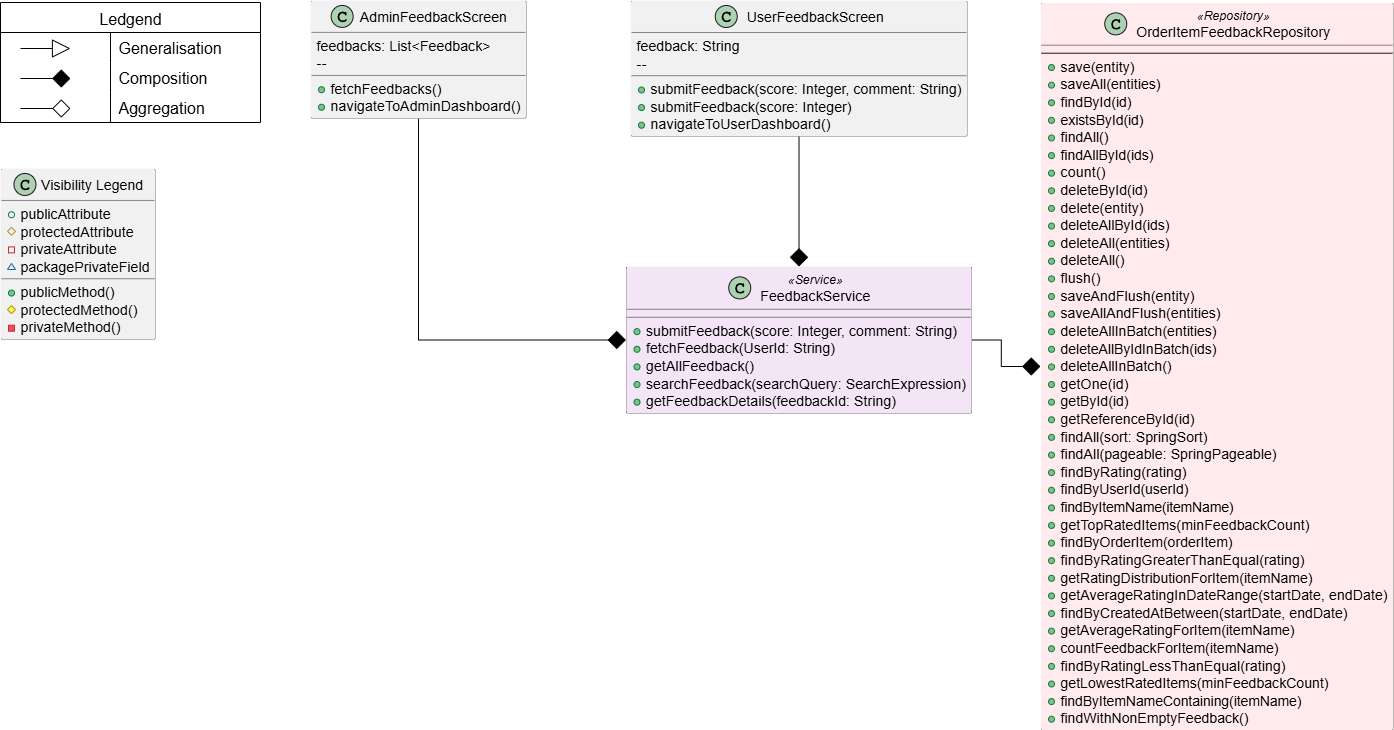
\includegraphics[width=\textwidth]{figures/class_diagrams/feedback-subsystem.png}
    \caption{Terugvoer onderdeel klasdiagram}
    \label{fig:feedback_subsystem_class_diagram}
\end{figure}

Hier volg die CRC kaarte vir die belangrikste klasse in hierdie
onderdeel.

\textbf{AdminFeedbackScreen} bied administrateurs 'n oorsig van alle terugvoer, insluitend statistieke en filterfunksies.
\begin{table}[H]
\centering
\begin{tabular}{|p{0.4\textwidth}|p{0.4\textwidth}|}
    \hline
    \multicolumn{2}{|c|}{\textbf{AdminFeedbackScreen}} \\
    \hline
    \textbf{Verantwoordelikhede} & \textbf{Medewerkers} \\
    \hline
    Wys alle terugvoer vir administrateurs \newline
    Verskaf terugvoer-statistieke en ontleding \newline
    Filter terugvoer volgens verskillende kriteria
    &
    FeedbackService \\
    \hline
\end{tabular}
\caption{CRC vir AdminFeedbackScreen}
\label{tab:crc_admin_feedback_screen}
\end{table}

\textbf{UserFeedbackScreen} verskaf die koppelvlak vir gebruikers om terugvoer te lewer, insluitend graderings en kommentaar.
\begin{table}[H]
\centering
\begin{tabular}{|p{0.4\textwidth}|p{0.4\textwidth}|}
    \hline
    \multicolumn{2}{|c|}{\textbf{UserFeedbackScreen}} \\
    \hline
    \textbf{Verantwoordelikhede} & \textbf{Medewerkers} \\
    \hline
    Verskaf vorm vir terugvoer \newline
    Valideer terugvoer-inligting \newline
    Dien terugvoer in op 5-punt skaal \newline
    Verskaf opsionele kommentaar
    &
    FeedbackService \\
    \hline
\end{tabular}
\caption{CRC vir UserFeedbackScreen}
\label{tab:crc_user_feedback_screen}
\end{table}

\textbf{FeedbackService} verwerk en stoor terugvoer, valideer insette, verskaf statistieke en koppel terugvoer aan bestellings.
\begin{table}[H]
\centering
\begin{tabular}{|p{0.4\textwidth}|p{0.4\textwidth}|}
    \hline
    \multicolumn{2}{|c|}{\textbf{FeedbackService}} \\
    \hline
    \textbf{Verantwoordelikhede} & \textbf{Medewerkers} \\
    \hline
    Verwerk en stoor terugvoer \newline
    Valideer terugvoer-inligting \newline
    Verskaf terugvoer-statistieke \newline
    Koppel terugvoer aan bestellings
    &
    OrderItemRepository \\
    \hline
\end{tabular}
\caption{CRC vir FeedbackService}
\label{tab:crc_feedback_service}
\end{table}